\documentclass[14pt]{extbook}
\usepackage{multicol, enumerate, enumitem, hyperref, color, soul, setspace, parskip, fancyhdr} %General Packages
\usepackage{amssymb, amsthm, amsmath, latexsym, units, mathtools} %Math Packages
\everymath{\displaystyle} %All math in Display Style
% Packages with additional options
\usepackage[headsep=0.5cm,headheight=12pt, left=1 in,right= 1 in,top= 1 in,bottom= 1 in]{geometry}
\usepackage[usenames,dvipsnames]{xcolor}
\usepackage{dashrule}  % Package to use the command below to create lines between items
\newcommand{\litem}[1]{\item#1\hspace*{-1cm}\rule{\textwidth}{0.4pt}}
\pagestyle{fancy}
\lhead{Progress Quiz 7}
\chead{}
\rhead{Version B}
\lfoot{3510-5252}
\cfoot{}
\rfoot{Summer C 2021}
\begin{document}

\begin{enumerate}
\litem{
Determine the vertical asymptotes and holes in the rational function below.\[ f(x) = \frac{9x^{3} +15 x^{2} -74 x + 40}{9x^{2} -9 x -10} \]\begin{enumerate}[label=\Alph*.]
\item \( \text{Vertical Asymptote of } x = 1.0 \text{ and hole at } x = 1.667 \)
\item \( \text{Vertical Asymptotes of } x = -0.667 \text{ and } x = 0.667 \text{ with a hole at } x = 1.667 \)
\item \( \text{Holes at } x = -0.667 \text{ and } x = 1.667 \text{ with no vertical asymptotes.} \)
\item \( \text{Vertical Asymptote of } x = -0.667 \text{ and hole at } x = 1.667 \)
\item \( \text{Vertical Asymptotes of } x = -0.667 \text{ and } x = 1.667 \text{ with no holes.} \)

\end{enumerate} }
\litem{
Determine the vertical asymptotes and holes in the rational function below.\[ f(x) = \frac{6x^{3} +37 x^{2} +75 x + 50}{8x^{2} +30 x + 25} \]\begin{enumerate}[label=\Alph*.]
\item \( \text{Vertical Asymptotes of } x = -1.25 \text{ and } x = -1.667 \text{ with a hole at } x = -2.5 \)
\item \( \text{Vertical Asymptotes of } x = -1.25 \text{ and } x = -2.5 \text{ with no holes.} \)
\item \( \text{Holes at } x = -1.25 \text{ and } x = -2.5 \text{ with no vertical asymptotes.} \)
\item \( \text{Vertical Asymptote of } x = -1.25 \text{ and hole at } x = -2.5 \)
\item \( \text{Vertical Asymptote of } x = 0.75 \text{ and hole at } x = -2.5 \)

\end{enumerate} }
\litem{
Which of the following functions \textit{could} be the graph below?
\begin{center}
    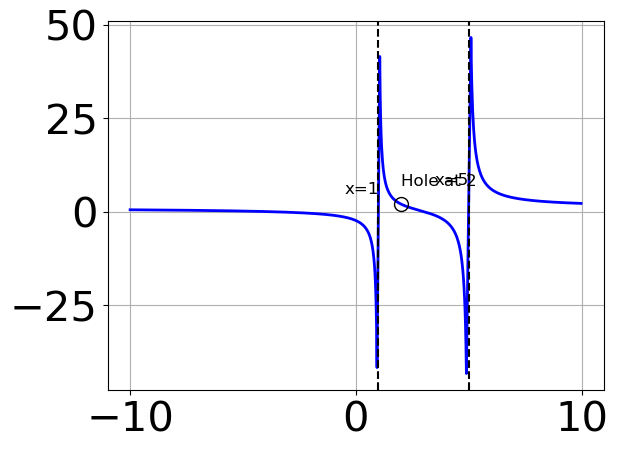
\includegraphics[width=0.5\textwidth]{../Figures/identifyGraphOfRationalFunctionCopyB.png}
\end{center}
\begin{enumerate}[label=\Alph*.]
\item \( f(x)=\frac{x^{3} +5.0 x^{2} -18.0 x -72.0}{x^{3} +8.0 x^{2} +17.0 x + 10.0} \)
\item \( f(x)=\frac{x^{3} -1.0 x^{2} -14.0 x + 24.0}{x^{3} -8.0 x^{2} +17.0 x -10.0} \)
\item \( f(x)=\frac{x^{3} + x^{2} -14.0 x -24.0}{x^{3} +8.0 x^{2} +17.0 x + 10.0} \)
\item \( f(x)=\frac{x^{3} +3.0 x^{2} -10.0 x -24.0}{x^{3} -8.0 x^{2} +17.0 x -10.0} \)
\item \( \text{None of the above are possible equations for the graph.} \)

\end{enumerate} }
\litem{
Determine the horizontal and/or oblique asymptotes in the rational function below.\[ f(x) = \frac{5x^{2} +23 x + 12}{15x^{3} -56 x^{2} +21 x + 36} \]\begin{enumerate}[label=\Alph*.]
\item \( \text{Horizontal Asymptote of } y = 0.333 \text{ and Oblique Asymptote of } y = 3x -25 \)
\item \( \text{Horizontal Asymptote of } y = 0 \)
\item \( \text{Horizontal Asymptote of } y = 0.333  \)
\item \( \text{Oblique Asymptote of } y = 3x -25. \)
\item \( \text{Horizontal Asymptote at } y = -4.000 \)

\end{enumerate} }
\litem{
Which of the following functions \textit{could} be the graph below?
\begin{center}
    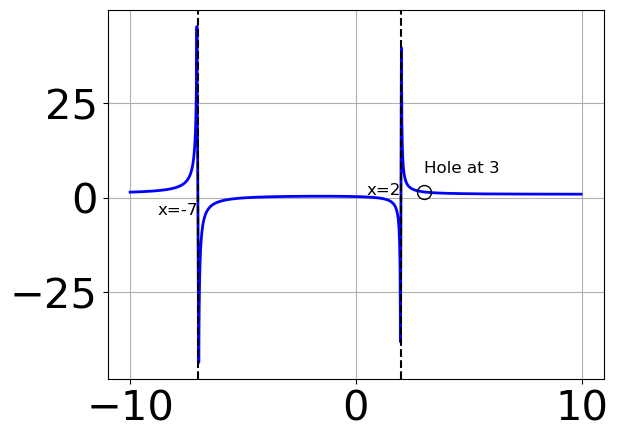
\includegraphics[width=0.5\textwidth]{../Figures/identifyGraphOfRationalFunctionB.png}
\end{center}
\begin{enumerate}[label=\Alph*.]
\item \( f(x)=\frac{x^{3} -1.0 x^{2} -17.0 x -15.0}{x^{3} -2.0 x^{2} -29.0 x -42.0} \)
\item \( f(x)=\frac{x^{3} +8.0 x^{2} +11.0 x -20.0}{x^{3} +2.0 x^{2} -29.0 x + 42.0} \)
\item \( f(x)=\frac{x^{3} +2.0 x^{2} -29.0 x -30.0}{x^{3} -2.0 x^{2} -29.0 x -42.0} \)
\item \( f(x)=\frac{x^{3} + x^{2} -17.0 x + 15.0}{x^{3} +2.0 x^{2} -29.0 x + 42.0} \)
\item \( \text{None of the above are possible equations for the graph.} \)

\end{enumerate} }
\litem{
Determine the vertical asymptotes and holes in the rational function below.\[ f(x) = \frac{4x^{3} -16 x^{2} -25 x + 100}{4x^{2} -4 x -15} \]\begin{enumerate}[label=\Alph*.]
\item \( \text{Vertical Asymptote of } x = 1.0 \text{ and hole at } x = 2.5 \)
\item \( \text{Vertical Asymptotes of } x = -1.5 \text{ and } x = 2.5 \text{ with no holes.} \)
\item \( \text{Holes at } x = -1.5 \text{ and } x = 2.5 \text{ with no vertical asymptotes.} \)
\item \( \text{Vertical Asymptotes of } x = -1.5 \text{ and } x = -2.5 \text{ with a hole at } x = 2.5 \)
\item \( \text{Vertical Asymptote of } x = -1.5 \text{ and hole at } x = 2.5 \)

\end{enumerate} }
\litem{
Determine the horizontal and/or oblique asymptotes in the rational function below.\[ f(x) = \frac{2x^{2} +9 x + 10}{12x^{3} -8 x^{2} -135 x -100} \]\begin{enumerate}[label=\Alph*.]
\item \( \text{Horizontal Asymptote of } y = 0.167  \)
\item \( \text{Horizontal Asymptote at } y = -2.000 \)
\item \( \text{Horizontal Asymptote of } y = 0.167 \text{ and Oblique Asymptote of } y = 6x -31 \)
\item \( \text{Oblique Asymptote of } y = 6x -31. \)
\item \( \text{Horizontal Asymptote of } y = 0 \)

\end{enumerate} }
\litem{
Determine the vertical asymptotes and holes in the rational function below.\[ f(x) = \frac{16x^{3} +16 x^{2} -9 x -9}{8x^{2} -14 x -15} \]\begin{enumerate}[label=\Alph*.]
\item \( \text{Vertical Asymptote of } x = 2.0 \text{ and hole at } x = -0.75 \)
\item \( \text{Vertical Asymptotes of } x = 2.5 \text{ and } x = 0.75 \text{ with a hole at } x = -0.75 \)
\item \( \text{Holes at } x = 2.5 \text{ and } x = -0.75 \text{ with no vertical asymptotes.} \)
\item \( \text{Vertical Asymptote of } x = 2.5 \text{ and hole at } x = -0.75 \)
\item \( \text{Vertical Asymptotes of } x = 2.5 \text{ and } x = -0.75 \text{ with no holes.} \)

\end{enumerate} }
\litem{
Determine the horizontal and/or oblique asymptotes in the rational function below.\[ f(x) = \frac{16x^{3} -16 x^{2} -25 x + 25}{4x^{2} -21 x + 20} \]\begin{enumerate}[label=\Alph*.]
\item \( \text{Horizontal Asymptote of } y = 4.0  \)
\item \( \text{Oblique Asymptote of } y = 4x + 17. \)
\item \( \text{Horizontal Asymptote at } y = 4.0 \)
\item \( \text{Horizontal Asymptote of } y = 4.0 \text{ and Oblique Asymptote of } y = 4x + 17 \)
\item \( \text{Horizontal Asymptote of } y = 4.0 \text{ and Oblique Asymptote of } y = 4x + 17 \)

\end{enumerate} }
\litem{
Determine the horizontal and/or oblique asymptotes in the rational function below.\[ f(x) = \frac{12x^{3} +11 x^{2} -45 x -50}{3x^{2} -7 x -20} \]\begin{enumerate}[label=\Alph*.]
\item \( \text{Horizontal Asymptote at } y = 4.0 \)
\item \( \text{Oblique Asymptote of } y = 4x + 13. \)
\item \( \text{Horizontal Asymptote of } y = 4.0  \)
\item \( \text{Horizontal Asymptote of } y = 4.0 \text{ and Oblique Asymptote of } y = 4x + 13 \)
\item \( \text{Horizontal Asymptote of } y = 4.0 \text{ and Oblique Asymptote of } y = 4x + 13 \)

\end{enumerate} }
\end{enumerate}

\end{document}